\section{Durchführung}
\label{sec:Durchführung}
Der Versuch wird wie in Abbildung \ref{fig:Vmi} vorbereitet. Jedoch wird an Stelle der an der Messzelle angebrachten Apparatur nur eine Handvakuumpumpe mit integriertem Manometer angeschlossen.
\begin{figure}
    \centering
    \caption{Versuchsaufbau Michelson-Interferometer \cite{v401}}
    \label{fig:Vmi}
    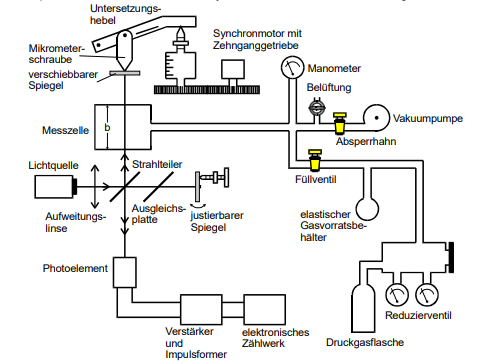
\includegraphics[width = 0.5 \textwidth]{pics/aufbauvv.png}
\end{figure}
Vor Benutzung des Interferometers muss es justiert werden. Dazu wird der Laser eingeschaltet.
Mit hilfe einer Hilfsmattscheibe, welche vor das Photoelement gehalten wird, werden die Strahlen sichtbar und können so am justierbaren Spiegel in Deckung gebracht werden.
Nach der Justierung kann das Michelson-Interferometer zur Wellenlängenbestimmung genutzt werden. Dazu wird der verschiebbare Spiegel mit einem Synchronmotor und einer Mikrometerschraube verbunden.
Zu beachten ist dabei, dass der Synchronmotor nicht zu schnell läuft, da sonst am Photoelement nicht alle Impulse erkannt werden. Es wird bei null Mikrometern begonnen zu messen, bis in etwa fünf Millimeter erreicht sind.
Danach werden die gemessenen Interfernzmaxima z am Zählwerk abgelesen. Danach wird die Laufrichtung des Motors umgestellt, so dass bei dem Zurücklaufen eine weitere Messung durchgeführt werden kann.
Die Prozedur wird weitere fünf mal wiederholt.
Um den Brechungsindex von Luft zu ermitteln wird der Synchronmotor ausgeschaltet. Die Messzelle wird über die Vakuumpumpe evakuiert und währenddessen wird die Messung der Intensitätsmaxima durchgeführt.
Der Druck $p$ in der evakuierten Messzelle wird am Manometer abgelesen. Danach wird das Ventil geöffnet und es werden erneut die Intensitätsmaxima gemessen.
Der Vorgang wird vier weitere male wiederholt.
